\documentclass[8pt]{beamer}

\setbeamertemplate{background canvas}[vertical shading][bottom=cyan!10,top=blue!10]

\usetheme{Warsaw}
\usefonttheme[onlysmall]{structurebold}

% pour le fichiers .pdf
\usepackage{graphicx}
\usepackage{color}
% pour les fichiers .png
% \usepackage{pgf,pgfarrows}
% \usepackage{pgf,pgfarrows}
\usepackage{amsmath,amssymb}
\usepackage[latin1]{inputenc}
\usepackage[T1]{fontenc}
\usepackage[french]{babel}
\usepackage{textcomp}
\usepackage{multitoc}
\usepackage{mdwtab}
\setbeamercovered{dynamic}
\DeclareMathOperator*{\argmin}{argmin}

\title[C++/Python binding]{C++/Python binding}
\author[R. Lebrun, copyright EADS 2011.]
{
  Trainer : R�gis LEBRUN, EADS/IW/SE/AM
  regis.lebrun@eads.net
}



\date[March 22-25th 2011]
{
  Developers training \\

  \begin{center}
    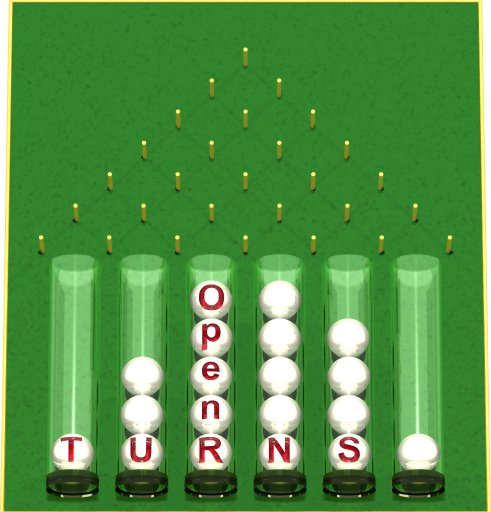
\includegraphics[height=2cm]{logoOT.jpg}
  \end{center}
}

\subject{OpenTURNS Developers Training}

% \part<presentation>{Corps de presentation}


\begin{document}

\frame{\titlepage}

% necessaire pour la table des matieres
\part{Main part}

% table des matieres
\begin{frame}
  \frametitle{C++/Python binding}
  \tableofcontents[part=1]
\end{frame}
%%%%%%%%%%%%%%%%%%%%%%%%% 
% The OpenTURNS package %
%%%%%%%%%%%%%%%%%%%%%%%%% 
\section[OpenTURNS TUI]{OpenTURNS Textual User Interface}
%%%%%%%%%%%%% 
% The tools %
%%%%%%%%%%%%% 
\begin{frame}
  \frametitle{OpenTURNS Textual Interface}
  \begin{block}{A user-friendly interface for the OpenTURNS library}
    OpenTURNS is intended to be used for complex industrial application. It means the ability to pilot complex simulation softwares, but also complex probabilistic modelling and involved strategies for uncertainty propagation. A typical graphical user interface does not provide the flexibility to address such needs, so OpenTURNS is proposed to the user as a Python module.\\
    Python is a full-featured object oriented programming language, and allows for complex scripting of functionalities comming from numerous modules. A typical uncertainty propagation study can be fully implemented using OpenTURNS only, but it can be easier to delegate some treatments to other graphical, statistical or numerical packages. For complex studies, it is the only way to do the job.\\
    The standard extension mechanisms proposed by Python to bind an external library are very low level mechanisms. It is mainly a C interface through which all the types are lost: the arguments are mainly {\ttfamily void *} pointers, and a lot of transtyping is required in order to make the things work.\\
    Several higher level tools have been developped in order to ease this binding, one of the most advanced being SWIG.
  \end{block}
\end{frame}

\begin{frame}
  \frametitle{SWIG: Simplified Wrapper and Interface Generator}
  \begin{block}{A tool to link C/C++ library with script languages}
    SWIG is a software development tool that connects programs written in C and C++ with a variety of high-level programming languages. SWIG is used with different types of target languages including common scripting languages such as Perl, PHP, Python, Tcl and Ruby. The list of supported languages also includes non-scripting languages such as C\#, Common Lisp (CLISP, Allegro CL, CFFI, UFFI), D, Go language, Java, Lua, Modula-3, OCAML, Octave and R. Also several interpreted and compiled Scheme implementations (Guile, MzScheme/Racket, Chicken) are supported. SWIG is most commonly used to create high-level interpreted or compiled programming environments, user interfaces, and as a tool for testing and prototyping C/C++ software. SWIG is typically used to parse C/C++ interfaces and generate the 'glue code' required for the above target languages to call into the C/C++ code.
  \end{block}
\end{frame}
\begin{frame}
  \frametitle{SWIG: Simplified Wrapper and Interface Generator}
  \begin{block}{Python, C++ and SWIG}
    Some of the (numerous) features of the C++ language have no equivalent in the Python language. Thus, there is a choice to be made on how to expose these features in Python. Two specific features are of interest in the OpenTURNS context:
    \begin{itemize}
    \item nested classes (a classe that is defined inside another class);
    \item parametric classes (no template concept in Python)
    \end{itemize}
    The new versions of SWIG (2.0.0 and later versions) are supposed to improve the support of these features, which means that they propose a standard way to expose these features without the help of the developer.\\
    Whereas it is often acceptable to abandon the nested classes in the C++ part without compromising too much the architecture, the parametric classes are more problematic. Some clues will be given in the development process part of this course.
  \end{block}
\end{frame}
\section[Development process]{Development process}
%%%%%%%%%%%%%%%%%% 
% Add a new class
%%%%%%%%%%%%%%%%%% 
\begin{frame}
  \frametitle{Integration of the new class in the TUI}
  \begin{block}{Step 9: create the SWIG interface file}
    In order to make the new class visible in the OpenTURNS Python module, you have to create a specific SWIG interface file, namely the file MyClass.i in the python/src directory. In most situations, it should be as simple as:
    \small
    \begin{tabular}{l}
      \ttfamily // SWIG file MyClass.i \\
      \ttfamily // Author : \$LastChangedBy: dutka \$ \\
      \ttfamily // Date : \$LastChangedDate: 2007-03-07 15:50:39 +0100 (mer. 07 mars 2007) \$ \\
      \ttfamily // Id : \$Id: Triangular.i 345 2007-03-07 14:50:39Z dutka \$ \\
      \ttfamily  \\
      \ttfamily \% \{ \\
      \ttfamily \#include "MyClass.hxx" \\
      \ttfamily \%\} \\
      \ttfamily  \\
      \ttfamily \%include MyClass.hxx \\
      \ttfamily namespace OpenTURNS \{ namespace NameSpace1 \{ namespace NameSpace2 \{ \\
      \ttfamily \%extend MyClass \{ MyClass(const MyClass \& other) \{ \\
      \ttfamily return new OpenTURNS::NameSpace1::NameSpace2::MyClass(other); \\
      \ttfamily \} \} \}\}\}
    \end{tabular}
    \normalsize
    supposing that your class is in the namespace {\ttfamily OpenTURNS::NameSpace1::NameSpace2}.
  \end{block}
\end{frame}
%%%%%%%%%%%%%%%%%% 
% Add a new class
%%%%%%%%%%%%%%%%%% 
\begin{frame}
  \frametitle{Integration of the new class in the TUI}
  \begin{block}{Step 11: integrate the SWIG interface file into the whole Python interface}
    \begin{itemize}
    \item Modify the Makefile.am file in python/src: add MyClass.i to the variable OPENTURNS\_SWIG\_SRC
    \item Locate in which of the Python submodule SWIG file you have to include MyClass.i (look for the file corresponding to the last level of namespace of your class)
    \end{itemize}
  \end{block}
\end{frame}
%%%%%%%%%%%%%%%%%% 
% Add a new class
%%%%%%%%%%%%%%%%%% 
\begin{frame}
  \frametitle{Integration of the new class in the TUI}
  \begin{block}{Step 12: test the new class in the Python module}
    \begin{itemize}
    \item Create a test file t\_MyClass\_std.py in the directory python/test. This test implements the same tests than t\_MyClass\_std.cxx, but using python.
    \item Create an autotest file t\_MyClass\_std.atpy that has the same role than t\_MyClass\_std.at, but for the python test.
    \item Modify the Makefile.am file in python/test:
      \begin{itemize}
      \item add t\_MyClass\_std.py to the variable PYTHONINSTALLCHECK\_PROGS. The several executables are organized following the library organization, you must follow this rule.
      \item add t\_MyClass\_std.atpy to the variable PYTHONINSTALLCHECK\_TESTS.
      \end{itemize}
    \end{itemize}
  \end{block}
\end{frame}
%%%%%%%%%%%%%%%%%% 
% Add a new class
%%%%%%%%%%%%%%%%%% 
\begin{frame}
  \frametitle{Integration of the new class in the TUI}
  \begin{block}{Step 12: document your new class in the TUI documentation}
    Comment your python test as a new use-case in the document\\ src/OpenTURNS\_UseCasesGuide/UseCasesGuide.tex following the generic format of this document:
    \begin{itemize}
    \item describe the inputs of your use-case.
    \item extract code snippets that show the user interaction with your class.
    \item add the relevant keywords to the index.
    \end{itemize}
    Gives a description of your class in the document src/UserManual/OpenTURNS\_UserManual.tex
    \begin{itemize}
    \item following the general form of this document, fill-in the sections but only describe the methods the user is intended to use (forget the most computer programming inclined methods).
    \item give some reminders of theoretical aspects if needed, in the form of an equation or a short (1 or 2 sentences) mathematical explanation. Give a pointer to the relevant reference guide section.
    \end{itemize}
  \end{block}
\end{frame}
%%%%%%%%%%%%%%%%%% 
% Add a new class
%%%%%%%%%%%%%%%%%% 
\begin{frame}
  \frametitle{Integration of the new class in the TUI}
  \begin{block}{Pitfalls, tips and tricks}
    Python does not support nested classes. As such, SWIG does  not propose any automatic mechanism to expose such classes in Python. The solution retained in OpenTURNS is to typedef the instanciations of the parametric classes to explicit new classes. Example:
    \begin{itemize}
    \item In the C++ library:
      \small
      \begin{tabular}{l}
        \ttfamily template <class T> class Collection \\
        \ttfamily typedef Collection< Distribution > DistributionCollection;
      \end{tabular}
      \normalsize
    \item In the SWIG interface file:
      \small
      \begin{tabular}{l}
        \ttfamily \% template(DistributionCollection) OpenTURNS::Base::Type::\\
        \ttfamily Collection<OpenTURNS::Uncertainty::Model::Distribution>;
      \end{tabular}
      \normalsize
    \end{itemize}
    For the nested classes, no reasonable solution has been found: we had to unnest the class in the SWIG interface file, creating C++ source code to be maintained in the SWIG interface. We decided to do this job in the C++ library instead.
  \end{block}
\end{frame}
%%%%%%%%%%%%%%%%%% 
% Add a new class
%%%%%%%%%%%%%%%%%% 
\begin{frame}
  \frametitle{Integration of the new class in the TUI}
  \begin{block}{Automatic conversion between C++ types into Python types}
    The automatic conversion of types is needed both to ease the writing of OpenTURNS scripts by Python users. Two distinct cases are of concern with OpenTURNS:
    \begin{itemize}
    \item The automatic conversion between Python lists/arrays and OpenTURNS collections;
    \item The automatic promotion of implementation classes into interface classes.
    \end{itemize}
    The first point is adressed both at the Python level and the C++ level:
    \begin{itemize}
    \item A set of parametric wrapping methods are defined in a C++ header (see PythonWrappingFunction.hxx in python/src);
    \item All the parametric classes are extended at the SWIG level with constructors from Python objects, using these wrapping methods.
    \end{itemize}
    The second point is due to the lack of capabilities of SWIG to identify correctly the Bridge pattern and use the existing constructors in order to perform the automatic conversions. It results in a need to make these conversions explicitely in the Python scripts, which is not natural for a Python programmer. The solution retained in OpenTURNS is to use the {\ttfamily typemap} service of SWIG and the wrapping methods in order to make these conversions automatic for the Python programmer (see Distribution.i in python/src).
  \end{block}
\end{frame}
\end{document}